\documentclass{article}
\usepackage{graphicx, verbatim, kotex} % Required for inserting images

\title{실습5}
\author{전형진 C011192}
\date{May 2024}
\begin{document}

\maketitle

\section{Prolog 과제}

\subsection{Prolog에 대하여}
프롤로그는 논리형 프로그래밍 언어이다. 논리식을 바탕으로 사실(Fact)과 사실을 이용하는 규칙들로 프로그램을 생성한다. 변수라는 기억공간의 추상화를 이용하는 명령형 언어와, 수학적 함수를 모델링한 함수형 언어와는 달리 오직 사실과 규칙을 이용한다는 점에서, 단지 주어진 코드로 동작한다는 사실을 넘어서 새로운 사실을 도출할 수 있다. 주어진 산술식을 계산한다는 느낌보다는 주어진 사실을 가지고 사실을 도출해내는 추론의 느낌으로 접근하면 좋다.
Prolog은 데이터는 Atom, 변수, 특수변수, 숫자, 리스트로 이루어져 있다. 여기서 변수는 명령형 언어에서 사용하는 기억공간의 추상화가 아니다. 단지 관계를 나타내는 일종의 규칙일 뿐이다. Prolog에서 중요한 것은 사실, 규칙, 그리고 질문이다. 이 세 요소는 추론형 언어인 Prolog의 전부라고 해도 과언이 아니다. 
\subsubsection{사실}
어떤 명세를 true라고 정의한 것이다. father(A, B) => A는 B이의 아버지이다.
\subsubsection{규칙}
정의한 사실을 가지고 변수를 이용해서 그들의 관계를 나타낸 것이다.
\subsubsection{질문}
나온 규칙을 가지고 새로운 규칙을 만들어 내거나 확인할 수 있는 질문을 할 수 있다.

\newpage
\section{전체적인 코드의 작동 설명 - InsertionSort}
\subsection{trace}
\begin{figure}[h]
    \centering
    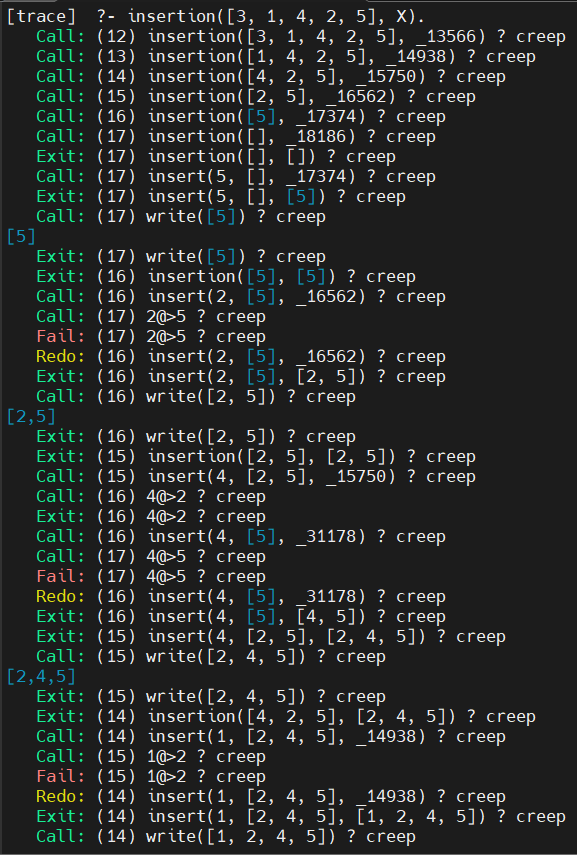
\includegraphics[scale = 0.7]{traceinsert1.png}
    \caption{insertion\_sort trace 실행모습}
\end{figure}
\begin{figure}[h]
    \centering
    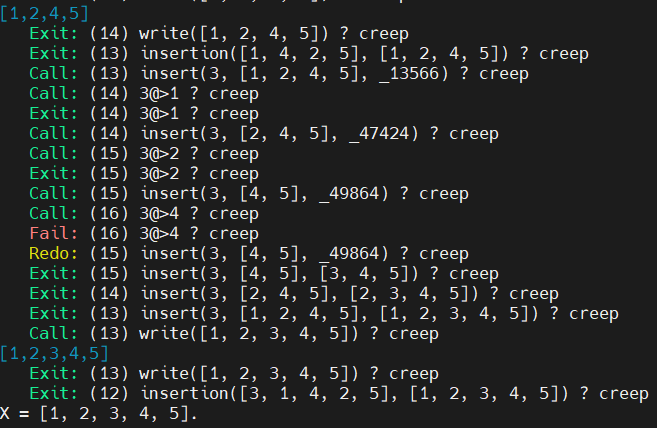
\includegraphics[scale = 0.7]{traceinsert2.png}
    \caption{insertion\_sort trace 실행모습}
\end{figure}

insertionsort는 처음 입력을 받은 리스트의 원소를 전부 다루기 위해 재귀를 이용해서 sublist로 분할한다. 마지막까지 남은 원소부터 원래 정렬하려고 하는 반환 리스트에 넣는다. 이때, 처음 넣는 원소를 제외한 나머지 원소들은 원래 있던 원소들과 대소 비교를 통하여 자신이 들어갈 위치를 직접 찾고 그 자리에 삽입이 된다.

\newpage

\subsection{코드 설명}
\begin{verbatim}
insertion([A|B], Sorted) :-
        insertion(B, SortedTail), % 입력받은 리스트를 전부다루기 위해 분할 하는 과정이다.
        insert(A, SortedTail, Sorted), % 입력 받은 리스트를 전부 분할했다면 insert 규칙으로 간다.
        write(Sorted).
insertion([], []).

insert(A, [B|C], [B|D]) :- % 여기서 원래 있던 원소들과 대소 비교를 통해 알맞은 자리에 삽입된다.
        A @> B, !,
        insert(A, C, D).
insert(A, C, [A|C]).

\end{verbatim}

\newpage

\subsection{실행결과}
\begin{figure}[h]
    \centering
    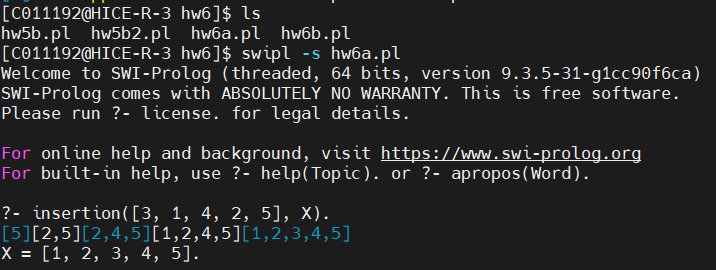
\includegraphics[scale = 0.7]{insert실행결과.png}
    \caption{insertion\_sort 결과}
\end{figure}

\subsection{어려웠던 점}
논리형 언어를 처음 사용하다보니 문법에 익숙하지 않았다. 처음 논리형 언어를 다뤘기 때문에 문법에 익숙해지는데 시간이 걸렸다. 논리형 언어 중 특히 prolog는 특정 규칙이 어떻게 사용되는지, 사실이 어디있는지 확인하기 헷갈렸다. 또한 리스트와 사실의 형태가 구분이 안되기 때문에 겉모습이 헷갈렸다. 디버깅하는데도 규칙과 관계가 생각이 나지 않아 무지하게 애를 먹었다.

\newpage

\section{전체적인 코드의 작동 설명 - N-queen}
\subsection{trace}
\begin{figure}[h]
    \centering
    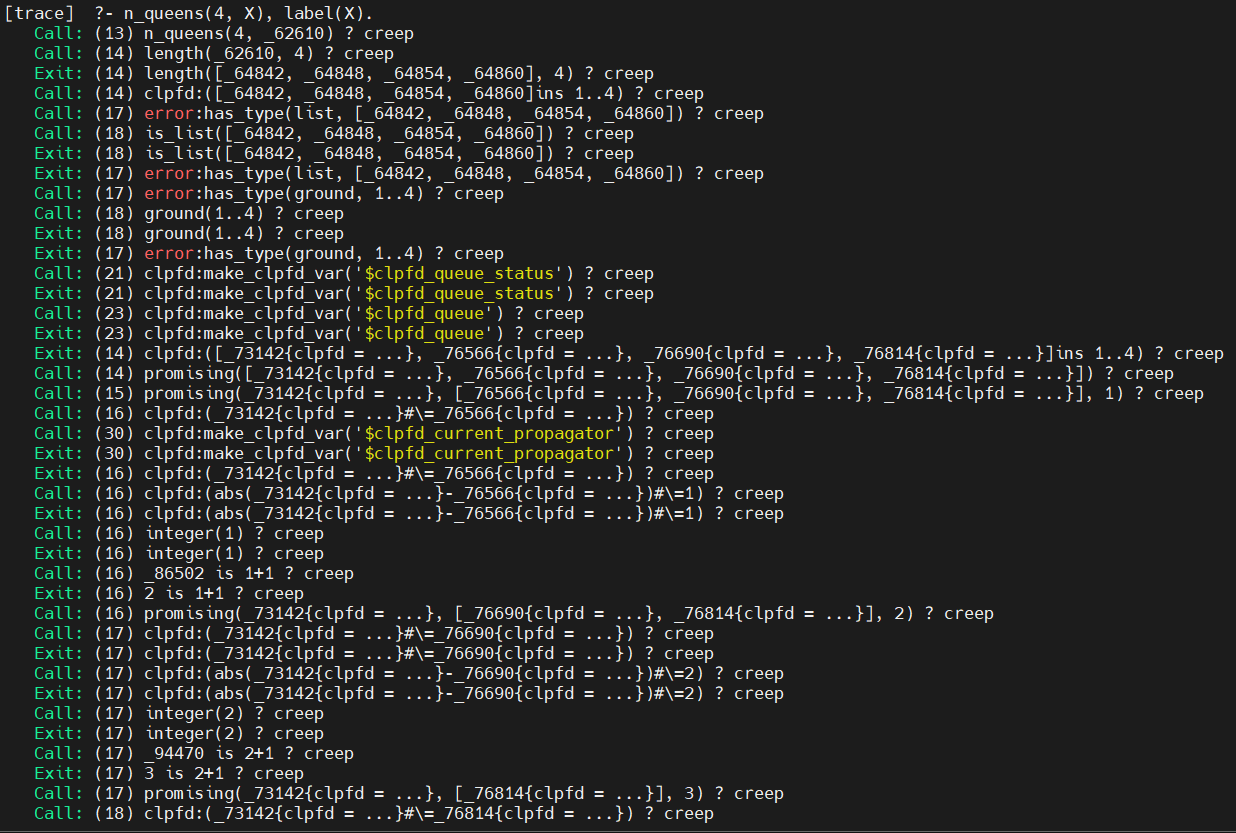
\includegraphics[scale = 0.7]{tracenqueens1.png}
    \caption{nqueen trace 실행모습}
\end{figure}
\begin{figure}[h]
    \centering
    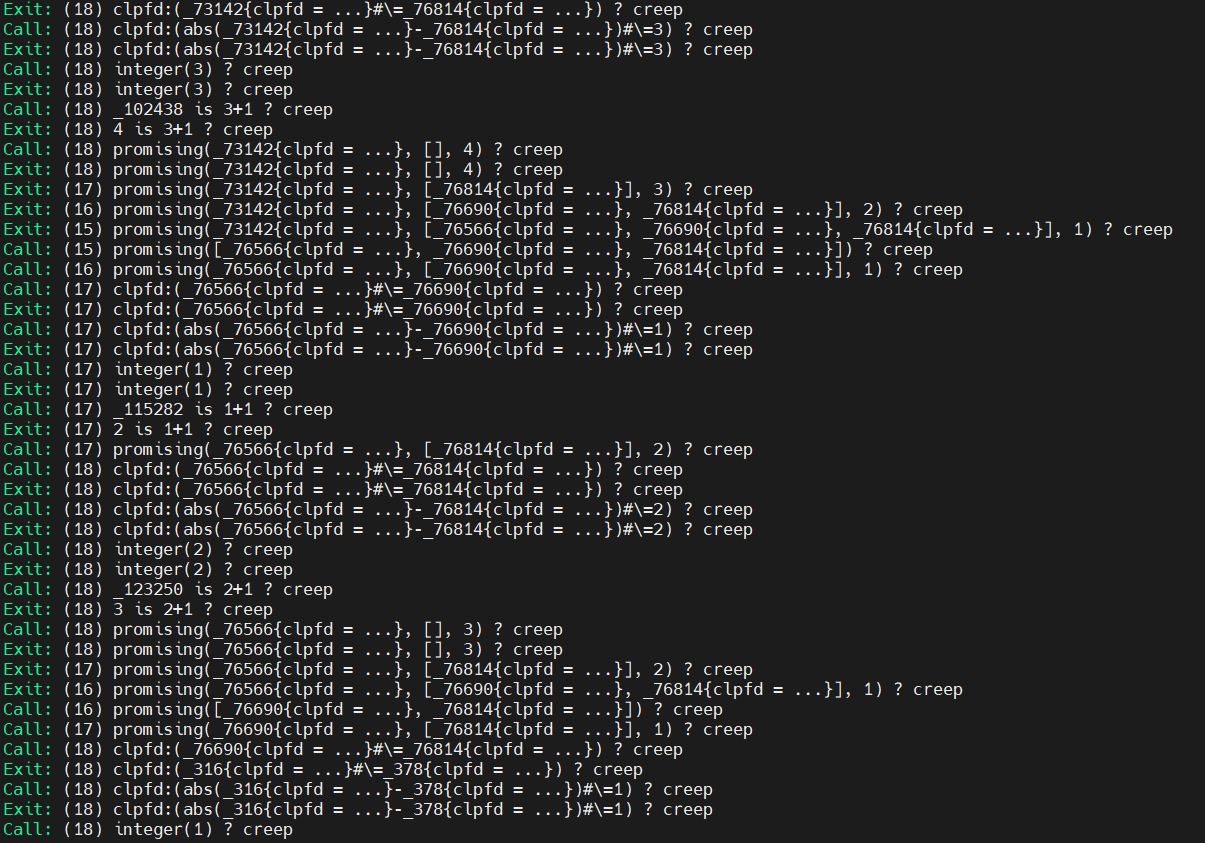
\includegraphics[scale = 0.7]{tracenqueens2.png}
    \caption{nqueen trace 실행모습}
\end{figure}
\begin{figure}[h]
    \centering
    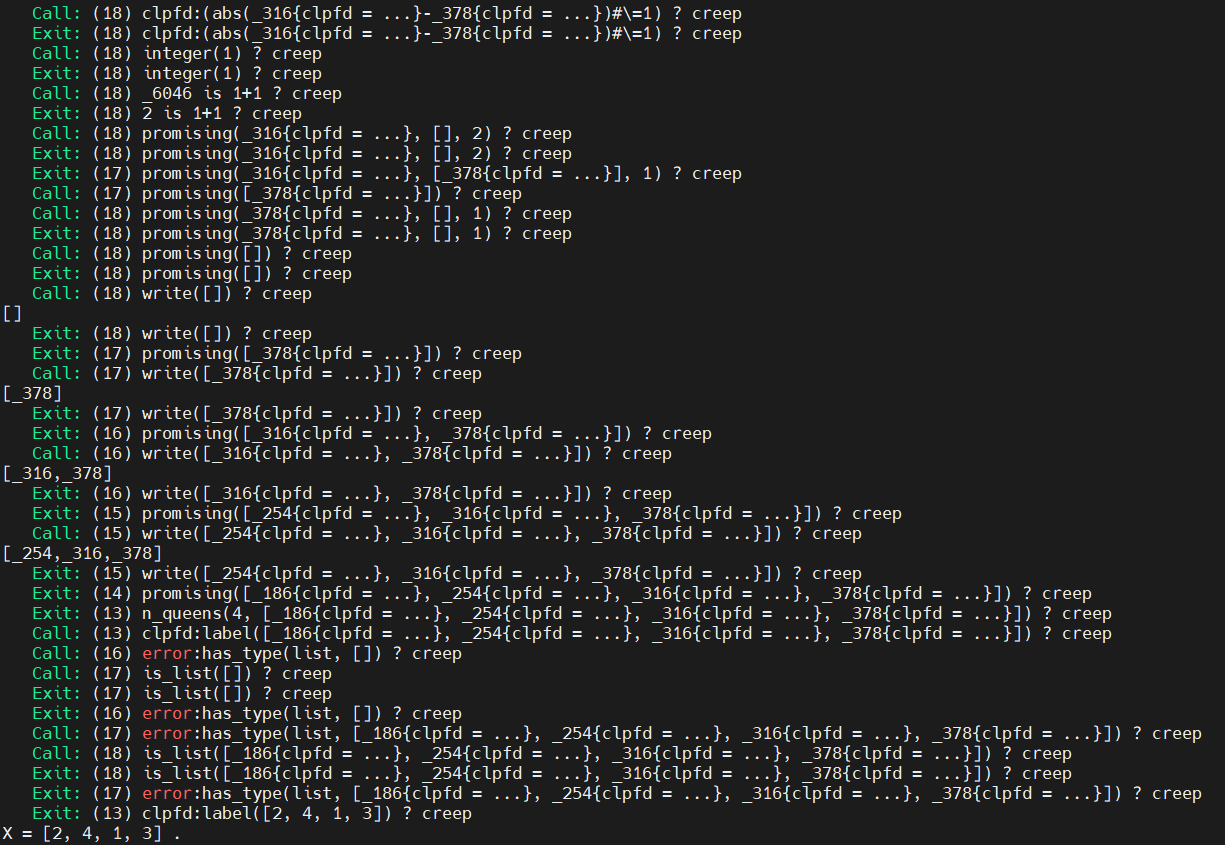
\includegraphics[scale = 0.7]{tracenqueens3.png}
    \caption{nqueen trace 실행모습}
\end{figure}

\newpage 

Prolog CLP(FD)가 제공하는 기능중 하나인 ins를 사용함에 따라 trace를 했을 때 코드의 가독성이 떨어진다. 그렇지만 하나씩 분석해보면, 우선 N값에 따라 N칸 짜리 빈 리스트를 생성한다. 빈 리스트를 생성하는 방법이 prolog에서는 정해져 있기 않기 때문에 ins를 사용한다. 만들어진 리스트를 바탕으로 ins 이용해 1부터 N까지의 수만 들어갈 수 있도록 만든다. 그 다음 원소 하나씩 넣으면서 col이 겹치지 않는지, diagonal이 겹치지 않은지 판단한다.

\newpage

\subsection{코드 설명}
\begin{verbatim}
:- use_module(library(clpfd)).

% 알고리즘 시작 부분
n_queens(N, Qs) :-
        length(Qs, N),
        Qs ins 1..N, % N칸 짜리 빈 리스트를 생성하고 각 칸의 한계 설정
        promising(Qs). % backtracking 방법 이용


promising([]). % 빈 리스트 도착 시 종료.
promising([Qf|Qs]) :- promising(Qf, Qs, 1), promising(Qs), write(Qs). % 리스트의 첫 번째 원소와 뒷 리스트로 나누고 검사. 재귀로 조각 낸 뒷 리스트도 검사.
promising(_, [], _).
% 첫 번째 원소와 뒷 리스트의 나머지 원소들 간의 적합성 판단.
promising(Qf, [Qf_lower|Qs_lower], Colik) :-
        Qf #\= Qf_lower, % 같은 행을 사용하고 있는지 검사.
        abs(Qf - Qf_lower) #\= Colik, % 같은 대각선에 있는지 검사.
        Colik_up #= Colik + 1,
        promising(Qf, Qs_lower, Colik_up). % 첫 번째 원소와 나머지 원소 들의 검사.

\end{verbatim}

\subsection{실행결과}
\begin{figure}[h]
    \centering
    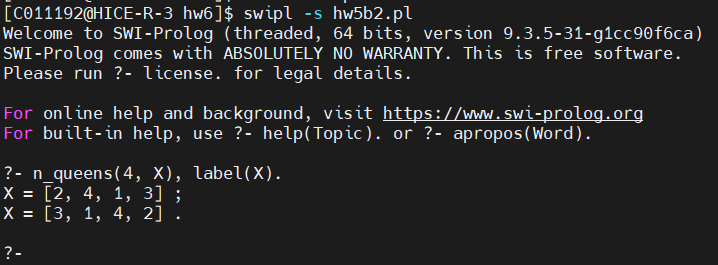
\includegraphics[scale = 0.7]{nqueens실행결과.png}
    \caption{nqueen 결과}
\end{figure}

\end{document}
